\section{Datenerstellung}
Die Bilder wurden am Nachmittag des 15.Januar mit einem Android Tablet erstellt.
Dieses enthält einen GPS-Sensor, sowie eine einfache Kamera.

\section{Probleme}
Beim Erstellen der Truth-Datensätze stellte sich heraus, dass der GPS-Sensor teilweise
ungenaue Positionen, welche um etliche Meter, wenn nicht sogar hunderte Meter von
der eigentlichen Position abweichen. Dieses ist im genauen Gegensatz zu den Testdatensätzen,
bei welchen die Bilder eine genauere Position lieferten, als es aus der Data.txt
herauszulesen war.

Als Lösung dieses Problems, wurde eine Überprüfung des Abstandes zwischen GPS-Koordinate
und Data.txt Koordinate implementiert, welche bei überschreiben eines Schwellwertes
die Koordinate im Bild verwirft. Es kann davon ausgegangen werden, dass Daten, welche
in die Data.txt eingetragen sind von Menschen überprüft wurden.


\section{Regelwerk}
\begin{figure}
  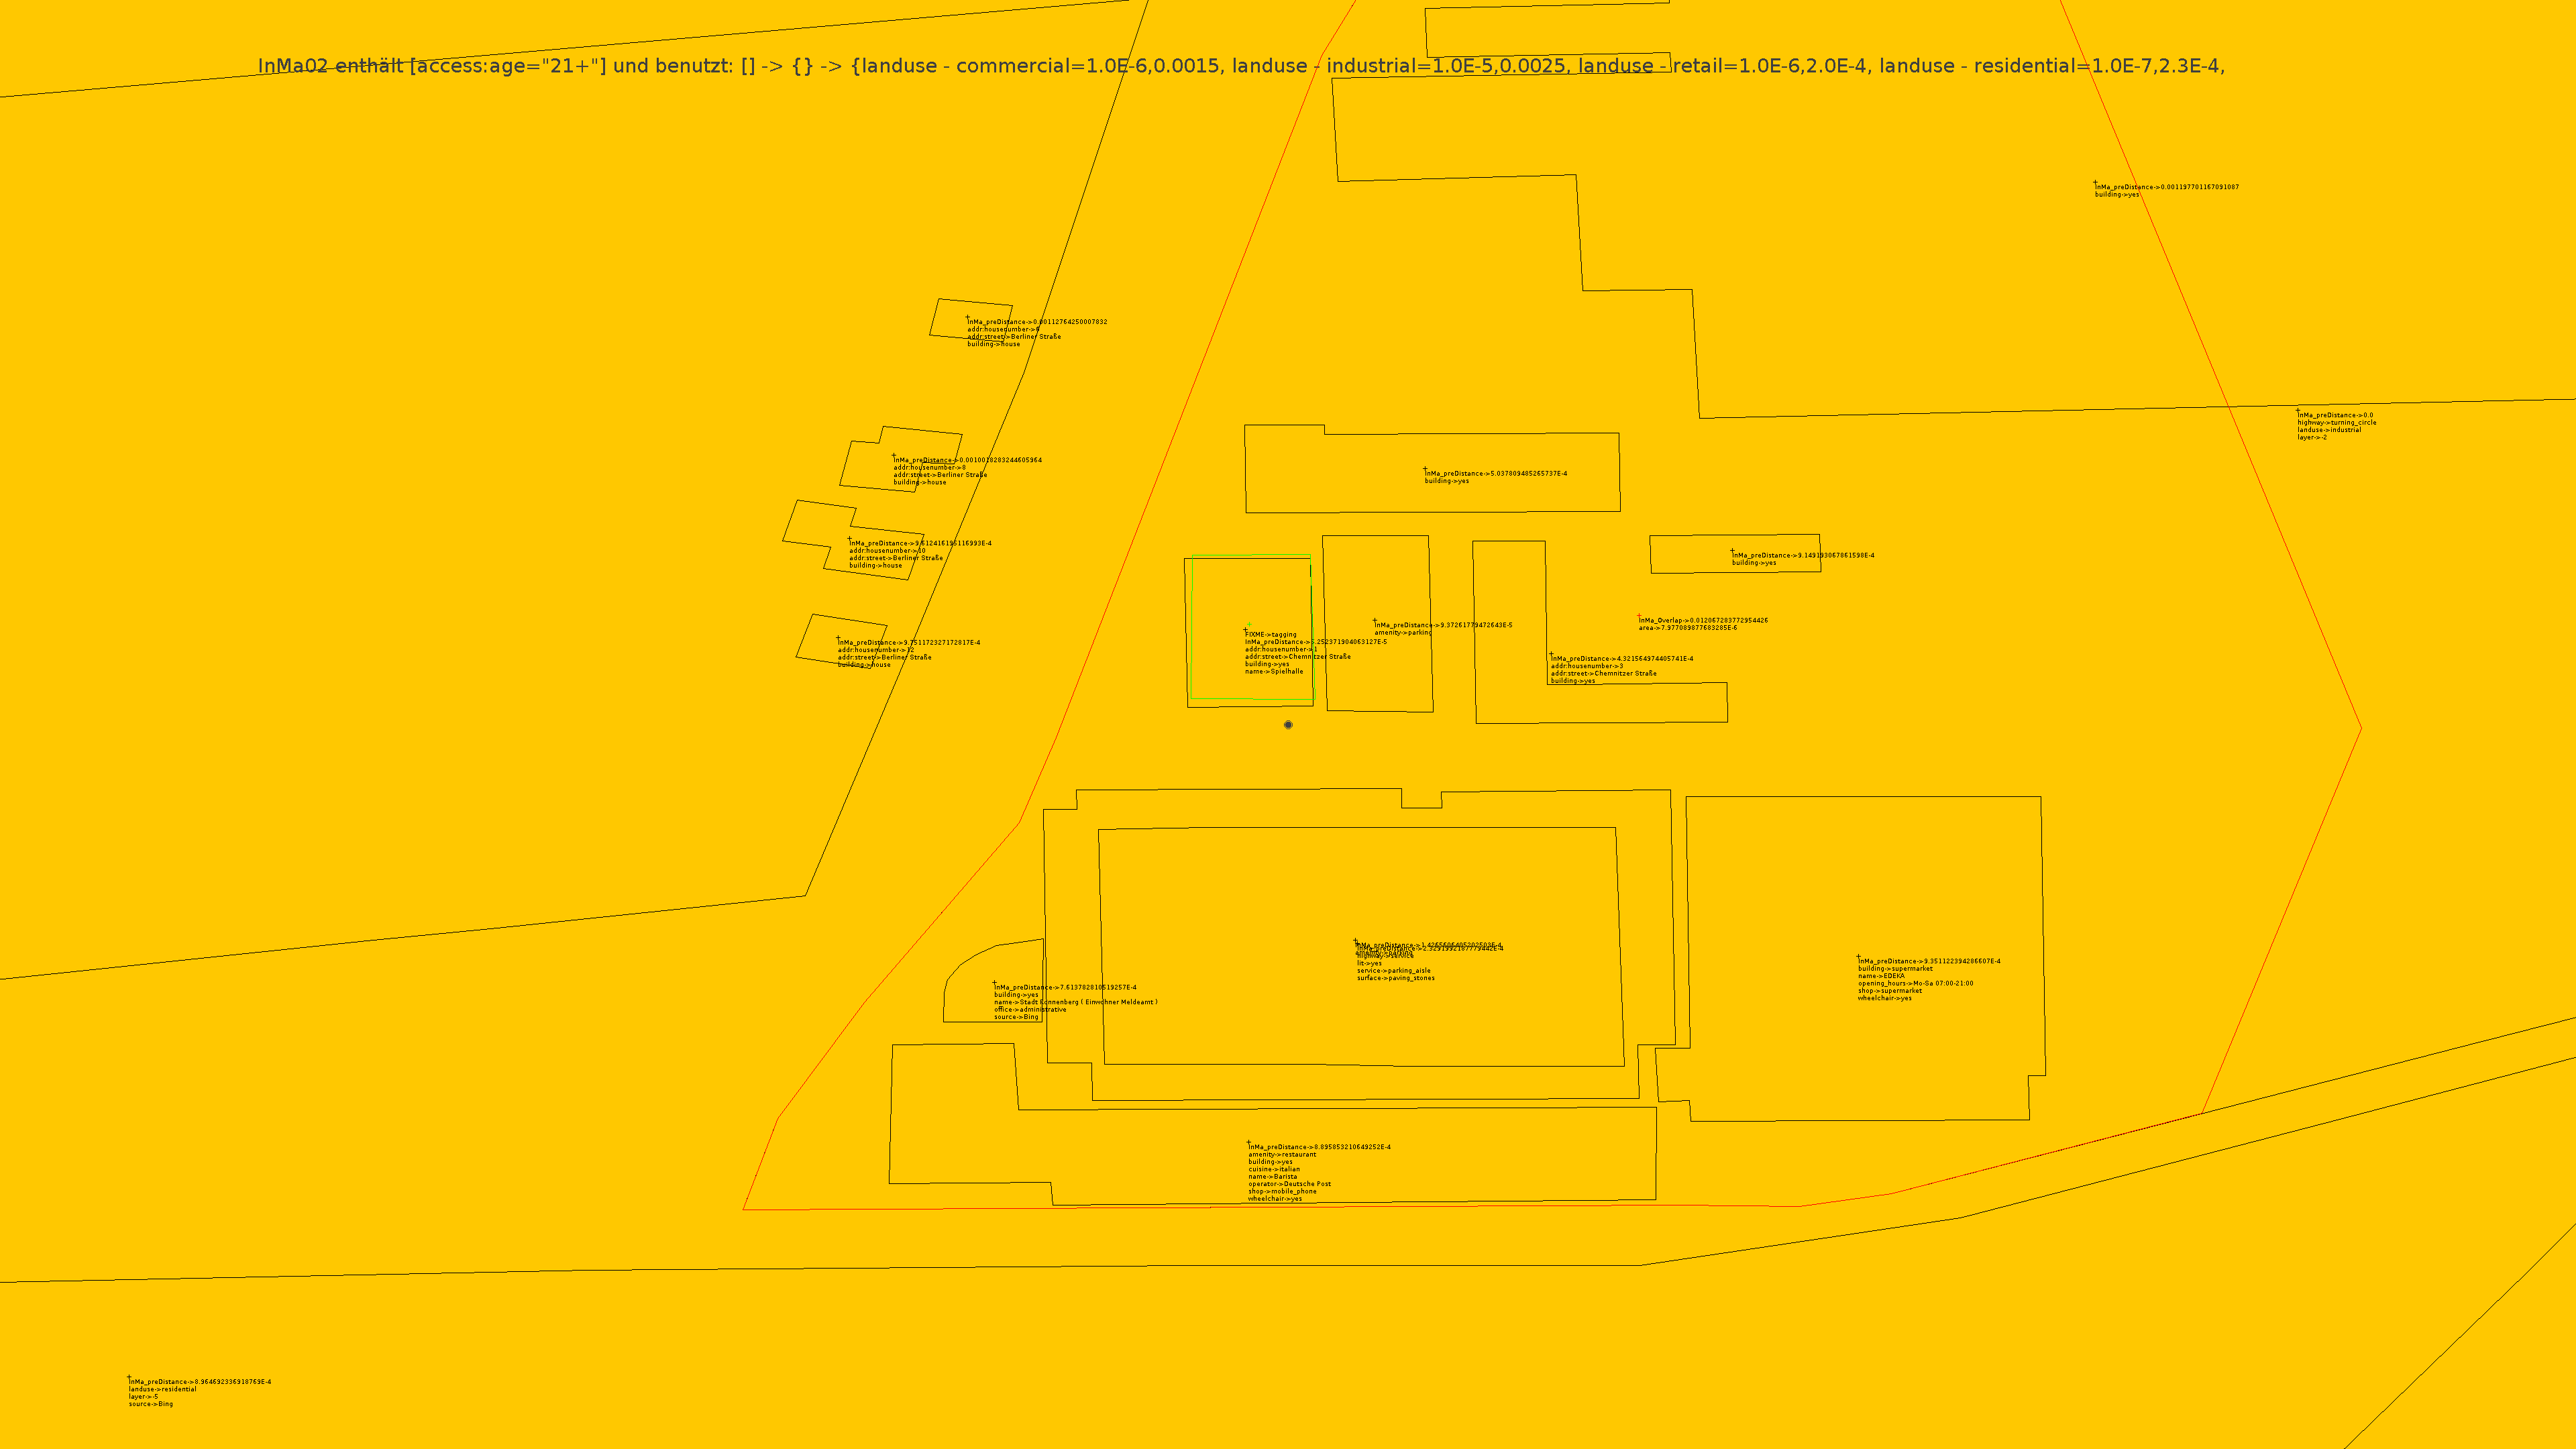
\includegraphics[width=\textwidth]{InMa02.png}
  \caption{Unvollständige Rules Definition.}
  \label{fig:NoRule}
\end{figure}

\begin{figure}
  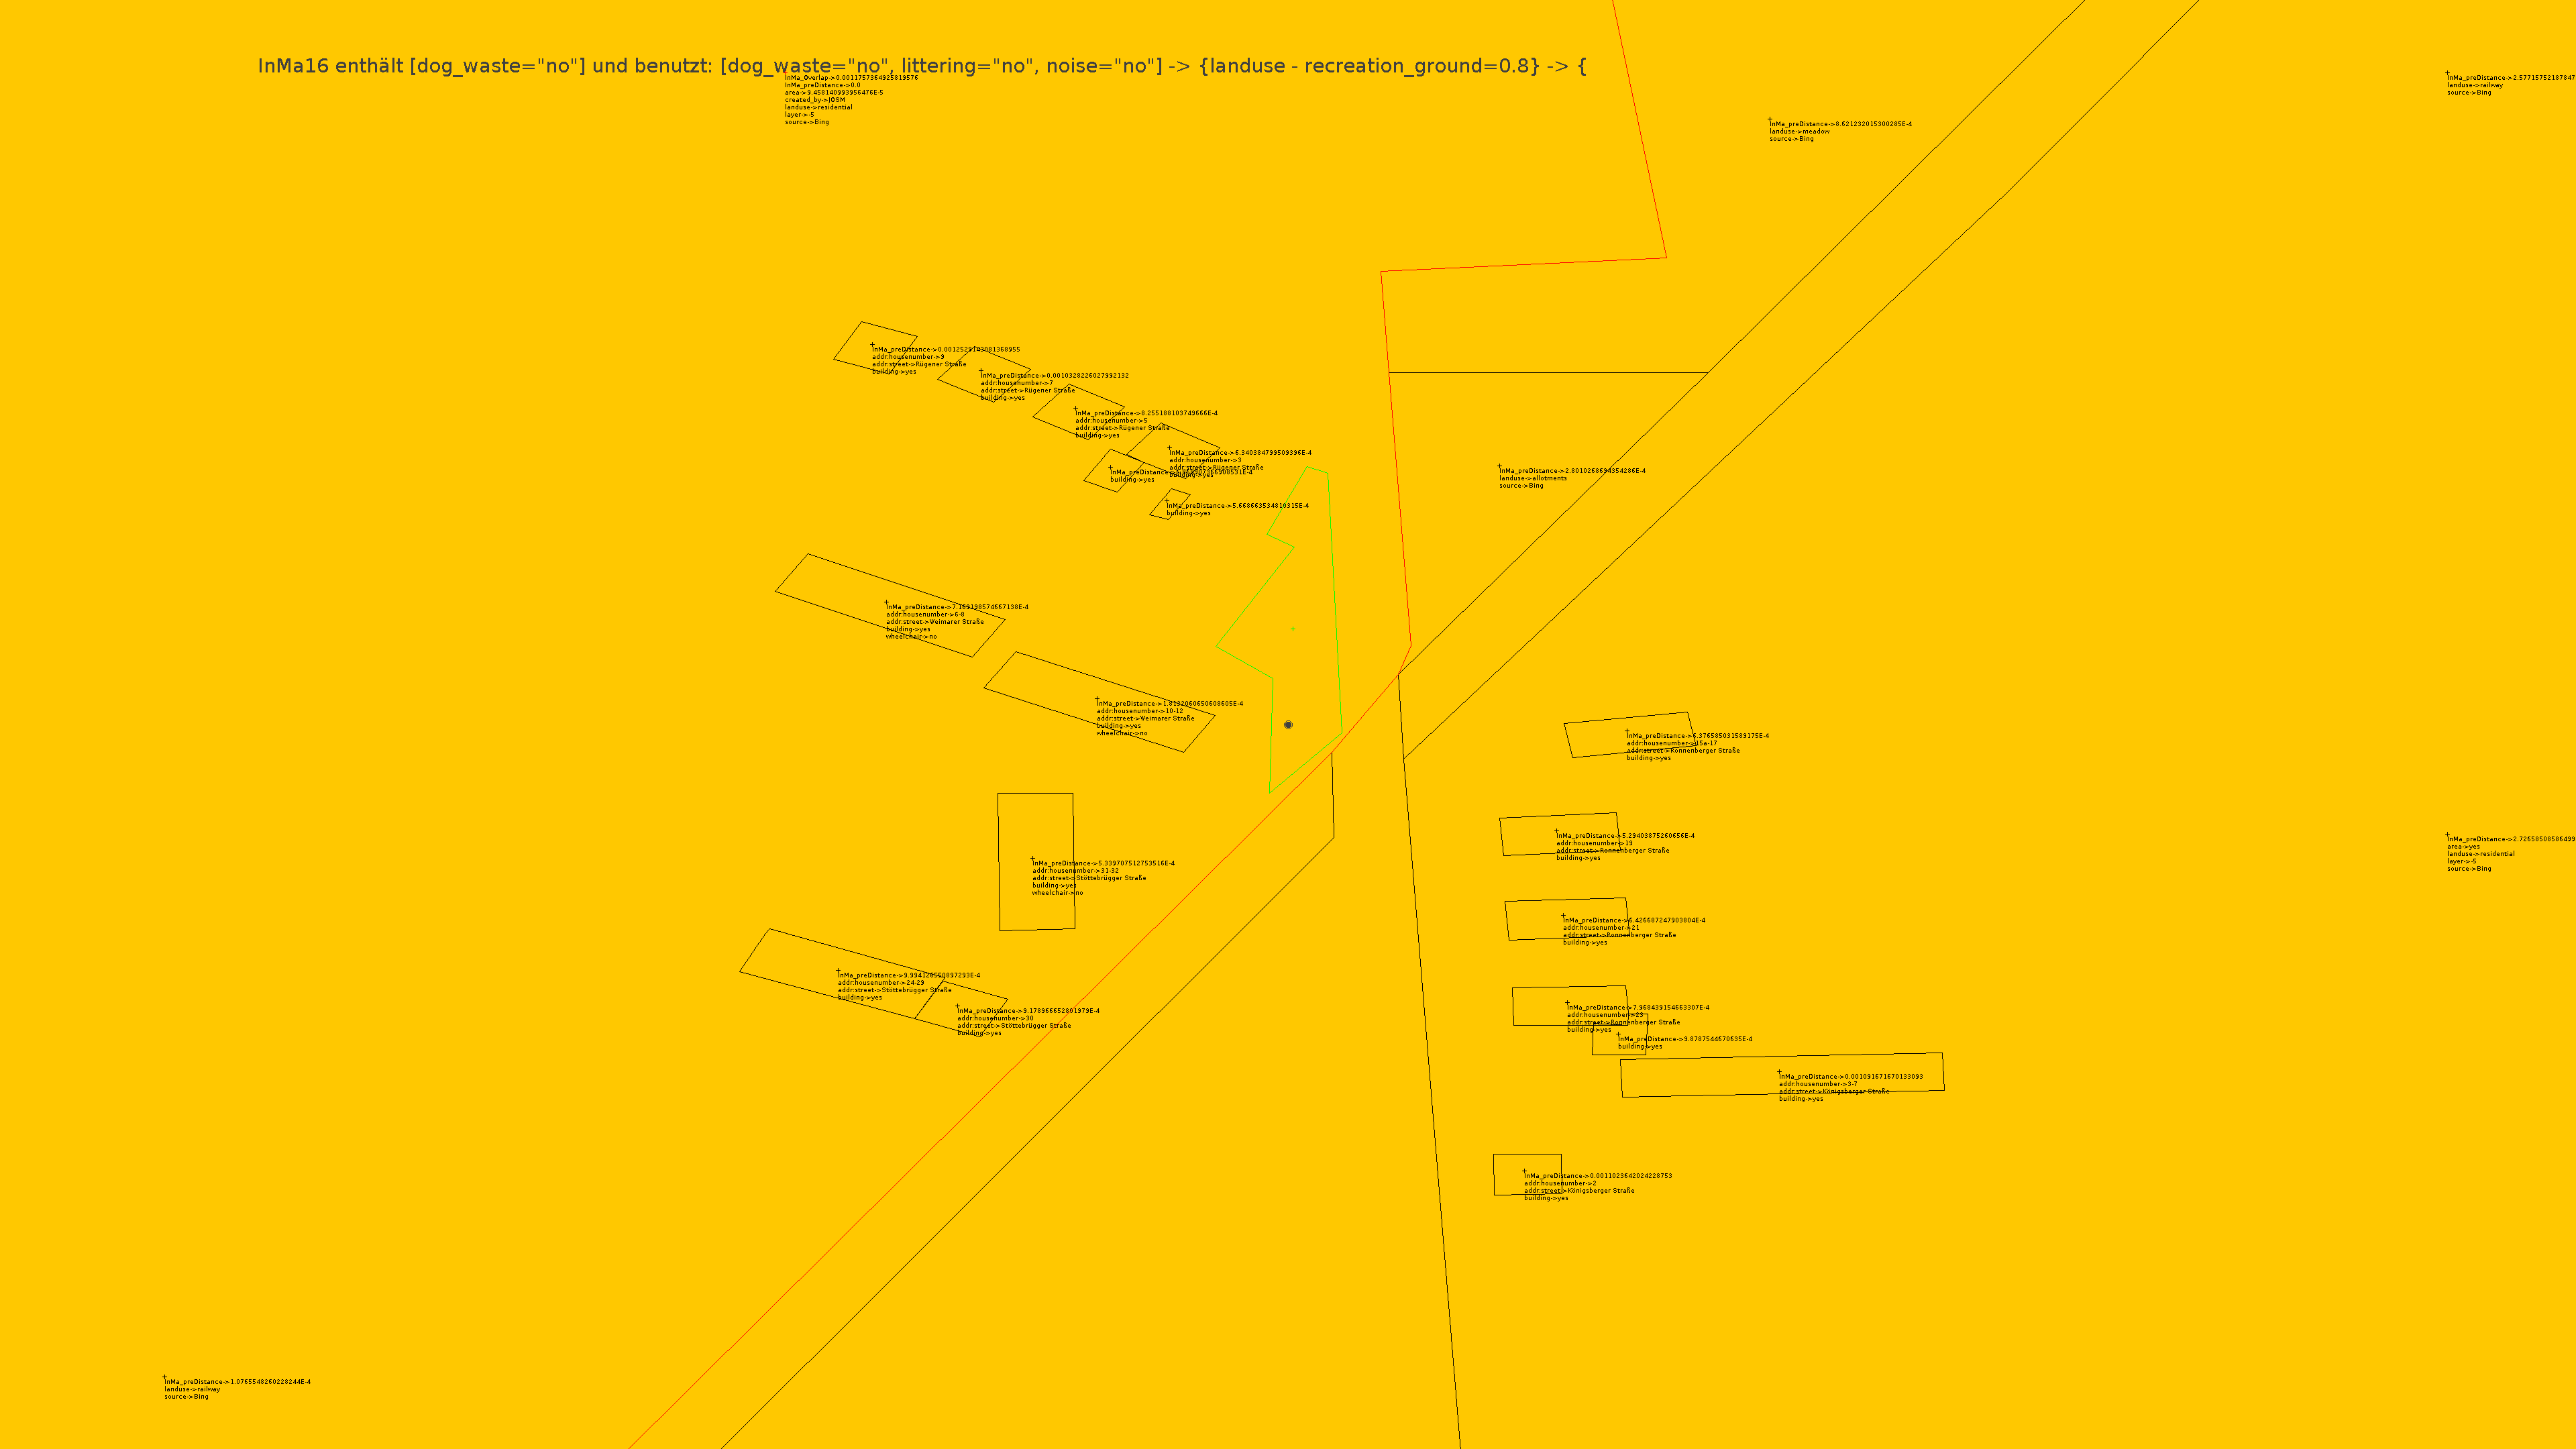
\includegraphics[width=\textwidth]{InMa16.png}
  \caption{Unvollständige Rules Einschränkungen.}
  \label{fig:MissingCircle}
\end{figure}
Das von uns bis jetzt definierte Regelwerk liefert nach einem ersten Durchlauf
zufriedenstellende Ergebnisse. Die Überlappungen sind meistens gegeben, jediglich
in 2 Fällen lag er komplett daneben. Dieses ist auf ein unvollständiges Regelwerk
aufgrund zu wenig Datansätzen zurück zu führen.

So gab es bis jetzt keine Definition für die Regel ''Zugang erst ab 21 Jahren''.
Dieses führte dazu, dass die Backup-Regel genommen wurde, das nächstebeste Polygon zu nehmen.
Da jedoch wie in \fref{fig:NoRule} zu sehen ist, das Bild vor dem gültigen Gebäude aufgenommen
wurde ist dem bisherigem Regelsatz nur noch die Regel:
\begin{lstlisting}[language=xml,frame=single]
<rule>
  <restriction>access:age="21+"</restriction>
  <OSMTag weight="0.7" >building</OSMTag>
</rule>
\end{lstlisting}
hinzuzufügen um auch diesen Datensatz vollständig zu bearbeiten.


Im zweiten Fall ist wie in \fref{fig:MissingCircle} zu sehen keine Representation
beabsichtigten Geltungsbereiches in OpenStreetMap vorhanden. Und auch wenn man davon
ausgehen kann, dass niemand gerne Hundkot vor der Nase hätte ist der beabsichtigte
Geltungsbereich für das Hinweisschild nur die Grünfläche, welche an den Parkplatz
und Strasse angrenzt.
Das Regelwerk ist also dahingehend zu ändern, dass folgende Regel hinzugefügt wird:
\begin{lstlisting}[language=xml,frame=single]
<rule>
  <restriction>dog_waste="no"</restriction>
  <OSMTag threshold="1e-8" radius="0.00023">landuse - residential</OSMTag>
</rule>
\end{lstlisting}
oder aber die bestehende Regel
\begin{lstlisting}[language=xml,frame=single]
<rule>
  <restriction>dog_waste="no"</restriction>
  <restriction>littering="no"</restriction>
  <restriction>noise="no"</restriction>
  <OSMTag weight="0.8" >landuse - recreation_ground</OSMTag>
</rule>
\end{lstlisting}
um den OSMTag erweitert wird.
Beides führt in diesem Fall zum gleichen Ergebnis.
